\section{Ziel}
Das Ziel dieses Versuchs ist es, mithilfe eines Michelson-Interferometers die Wellenlänge des von einem Laser emittierten Lichtes und durch Druckänderung den Brechungsindex von Luft zu bestimmen.

\section{Theorie}
\label{sec:Theorie}

\subsection{Interferenz}
Licht kann als ebene, elektromagnetische Welle beschrieben werden.
Interferenz ist die Überlagerung bei Zusammentreffen mehrerer Wellenzüge.
Aus der Interferenz kann beispielsweise die Wellenlänge des Lichtes berechnet werden.

% Licht kann als ebene, elektromagnetische Welle beschrieben werden
% \begin{equation*}
%     \var{E}= \var{E}_0 cos(kx - \omega t - \delta).
%     \label{eqn:efeld}
% \end{equation*}
% Dabei ist $x$ die Ortskoordinate, $k$ die Wellenzahl, $\omega$ die Kreisfrequenz und $\delta$ 
% die Phasenverschiebung. 

%\noindent Da sich Licht als Maxwellgleichung beschreiben lässt, gilt das Superpositionsprinzip. 
%Daher ist das elektrische Feld eines Lichtstrahls meist die Summe der Felder mehrerer 
%Lichtwellen.
%Dies lässt sich aber nicht unmittelbar nachprüfen. 
%Doch man kann die Intensität $I$ bestimmen. 

\noindent Die Lichtintensität lässt sich als
\begin{equation}
    I = const \, \abs{\vec{E}}^{2}
    \label{eqn:intensität}
\end{equation} 
formulieren.

% \noindent Aus der Kombination des Superpositionsprinzips von Wellen und der Gleichung 
% \ref{eqn:intensität} folgt, dass die Lichtintensität insgesamt an einem bestimmten Ort 
% $x$, durch
% \begin{equation}
%     I_\text{ges}= \frac{const}{t_2-t_1} int[t_1]{t_2} \l(\abs{\vec{E}_1 + \vec{E}_2} \r)^2 (x, t) dt
%     \label{eqn:iges}
% \end{equation}
% beschrieben wird. Dabei entsprechen die beiden $E$-Felder den in Gleichung \ref{eqn:efeld} 
% beschriebenen Zusammenhängen. 
% Durch das Einsetzen dieser beiden Terme entsteht zusätzlich zu der Summe der 
% Einzelintensitäten noch ein Teil 
% \begin{equation}
%     2 const \vec{E}_{0}^2 cos(\delta_2 - \delta_1).
%     \label{eqn:zusatz}
% \end{equation}
% Die Gesamtintesität kann um diesen Faktor von der Summe der Einzelintensitäten 
% abweichen. Im Fall, dass 
% \begin{equation}
%     \delta_2 - \delta_1 = (2n +1) \pi , n= 0, 1, 2, ...
% \end{equation}
% ist, verschwindet die Gesamtintensität sogar komplett. 

\subsection{Kohärenz}
\subsubsection{Kohärentes Licht}
%inkohärent
Inkohärentes Licht ist nicht interferenzfähiges Licht. Dieses Licht wird von zwei
verschiedenen Punkten einer Lichtquelle oder von zwei Lichtquellen emittiert.
\newline
%kohärent
Kohärentes Licht kann beispielsweise durch Laser (= light amplification by stimulated emisson of radiation)
erzeugt werden. Atome emittieren hierbei in konstantem Abstand Licht, sodass dieses 
kohärent ist.
\newline
%kohärentes Licht erzeugen
Eine andere Möglichkeit kohärentes Licht zu erzeugen ist, das Licht aus einer Quelle
mit einem Strahlteiler in zwei räumlich getrennte Strahlbündel aufzuteilen.
Durch Spiegel können die Bündel wieder zusammengeführt werden.
% Je nach Phasenverschiebung an diesem Punkt 
% verschwindet dann zum Beispiel die Lichtintensität an diesem Punkt, vorausgesetzt, dass 
% der Gangunterschied beträgt $\lambda/2$ und die Feldstärke beträgt in beiden Bündeln 
% dieselbe Größe.

\subsubsection{Kohärenzlänge und -zeit}
% Der Emissionsakt dauert nur eine endliche Zeit $\tau$, weshalb der Wellenzug auch nur 
% eine endliche Länge besitzt. Ist der Gangunterschied zwischen den Wellen deutlich größer 
% als diese Länge, so verschwindet die Interferenzerscheinung. Daher dürfen die 
% Wegunterschiede zwischen den Teilbündeln nicht zu groß werden. Die Länge, bei der die 
% Erscheinungen so eben verschwinden, nennt man Kohärenzlänge $l$. 
Die Kohärenzlänge ist der Wegunterschied, bei dem die Interferenzerscheinungen
gerade verschwinden:
\begin{equation*}
    l = z \lambda.
\end{equation*}
Dabei entspricht $z$ der Anzahl der am Schnittpunkt der Strahlen entstehenden Intensitätsmaxima 
und $\lambda$ der Wellenlänge des Lichts. 
Der Gangunterschied darf also nicht größer als $l$ sein.
\newline
Die Kohärenzzeit ist durch
\begin{equation*}
    \tau = \frac{l}{c}
\end{equation*}
gegeben, wobei $c$ der Lichtgeschwindigkeit entspricht.

%Fouriersches Theorem
%Aus dem Fouriersche Theorem folgt, dass ein Wellenzug endlicher Länge nicht 
%monochromatisch sein kann, sondern ein Frequenzspektrum besitzen muss. Somit muss 
%entweder der Gangunterschied so klein sein oder das Frequenzspektrum so schmal, dass 
%Maximum- und Minimumsbedingung für zwei Wellenlängen nicht am selben Ort realisiert werden 
%können. 

\subsubsection{Kohärenzbedingung} %wichtig?
Eine Bedingung für Interferenzerscheinungen ist, dass bei ausgedehnten 
Lichtquellen die Richtungsänderung $\zeta$ 
klein gegenüber $\pi$ sein muss. Es gilt also die Bedingung 
\begin{equation*}
    a \, sin(\zeta) << \frac{\lambda}{2}.
\end{equation*}

% \subsubsection{Polarisation}
% Interferenzerscheinungen bei linear polarisierten Teilbündeln
% können nur bei nicht senkrecht zueinander polarisierten Teilbündeln auftreten. 

\subsection{Das Michelson-Interferometer}
Ein Interferometer ist ein Gerät, das unter Ausnutzung von Interferenzeffekten die 
Messung optischer Größen erlaubt. 
Es wird mithilfe einer semipermeablen Platte $P$ ein Lichtstrahl in zwei Teilbündel 
gespalten. Anschließend wird eines der Bündel verändert, also es wird ein Gangunterschiedmhinzugefügt. Durch Spiegel werden die Bündel wieder zusammengeführt. Diese treffen auf den Detektor $D$.
Es ist nötig, eine Kompensationsplatte einzufügen, damit die Bündel die gleiche Strecke
durchlaufen.
Mit der in Abb. \ref{abb:michelson} dargestellten Apparatur kann die Intensität am 
Detektor $D$ gemessen werden. Dadurch lässt sich durch Variation des Abstandes $d$ eines Spiegels feststellen, an welchen Stellen die Maxima liegen. Dadurch widerum lässt sich die 
Wellenlänge $\lambda$ mit 
\begin{equation}
    \Delta d = z \cdot \frac{\lambda}{2}
    \label{eqn:lambda}
\end{equation}
berechnen. Dabei ist $z$ die Anzahl der Intensitätsmaxima.

\begin{figure}
    \centering
    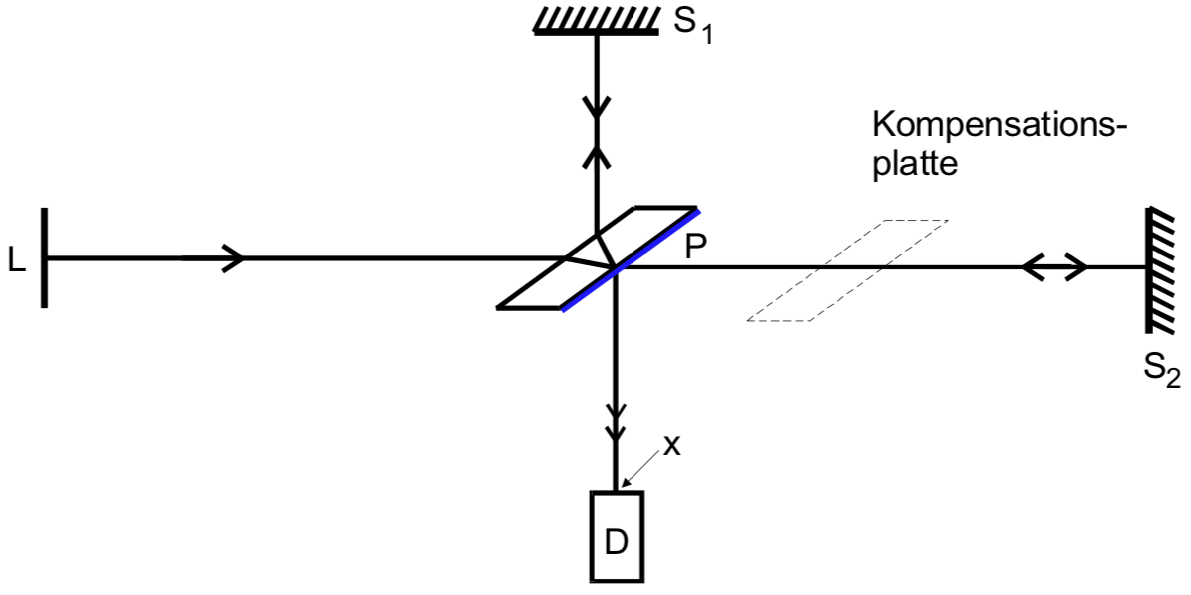
\includegraphics[width=12cm, height=6cm]{build/michelson.png}
    \caption{Es ist der Aufbau des Michelson-Interferometers zu sehen. Dabei ist $L$ der Laser, $P$ die semipermeable Platte, $S_1$ und $S_2$ sind Spiegel und $D$ ist der Detektor. Außerdem ist eine Kompensationsplatte zu sehen. Die Strahlwege sind durch die Linien und die Richtung durch die Pfeile gekennzeichnet. \cite{V401}}
    \label{fig:michelson}
\end{figure}

\noindent Alternativ wird ein Medium mit geändertem Brechungsindex mit einer Breite $b$ eingesetzt.
Diese Apparatur ist in Abb. \ref{fig:michelson2} zu sehen.
Bei Änderung des Gasdrucks gilt
\begin{equation}
    b \cdot \Delta n = z \cdot \frac{\lambda}{2}.
    \label{eqn:deltan}
\end{equation}
Da $\lambda$ im Allgemeinen deutlich kleiner als $b$ ist, lässt sich damit ein 
Unterschied des Brechungsindex in der Größenordnung von $\num{10e-5}$ bestimmen.

\noindent Der Brechungsindex unter Normalbedingungen ist durch
\begin{equation}
    n(p_0, T_0) = 1 + \Delta n(p,p') \, \frac{T}{T_0} \, \frac{p_0}{p - p'}
    \label{eqn:n}
\end{equation}
gegeben. Hier ist $T$ die Temperatur, $p$ der Innendruck und $p'$ ein kleinerer Druck.
Die Normalbedingungen sind
\begin{align*}
    p_0 &= \SI{1013.2}{\milli\bar} \\
    T_0 &= \SI{273.15}{\kelvin}.
\end{align*}

\begin{figure}
    \centering
    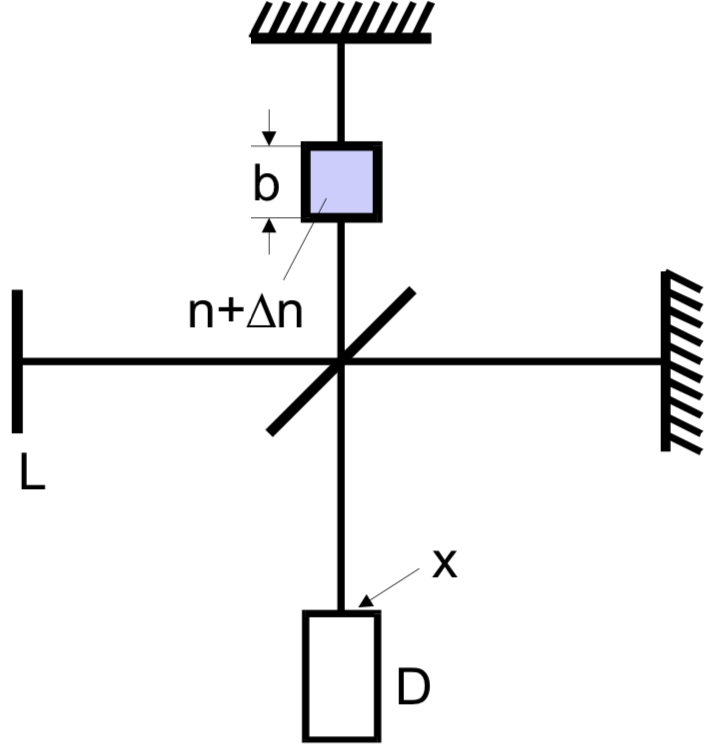
\includegraphics[width=6cm, height=7cm]{build/michelson2.png}
    \caption{Es ist der Aufbau des Michelson-Interferometers mit zusätzlichem Medium mit einem unterschiedlichem Brechungsindex zu sehen. Der Laser, die semipermeable Platte, die Spiegel und der Detektor bleiben unverändert. \cite{V401}}
    \label{fig:michelson2}
\end{figure}

% Da divergente Strahlbündel genutzt werden, kann der Wegunterschied auch noch vom Winkel 
% zwischen der Spiegelnormalen und der Einfallsrichtung des Strahls abhängen. Für eine 
% Veränderung des Winkels $\alpha$ können ebenso mehrere Maxima festgestellt werden. 
% Diese befinden sich bei 
% \begin{equation}
%     cos (a_k)= \frac{k \lambda}{2 d} (k= 1, 2, ..., \frac{2d}{\lambda}).
% \end{equation}
% Dabei wird ein System konzentrischer Kreise am Detektor betrachtet. Diese werden 
% Interferenzkurven gleicher Neigung genannt. 

% \subsection{Fourier-Spektroskopie}

% Mit dem Fourierschen Theorem 
% \begin{equation}
%     G(k)= \frac{1}{2\pi} \int{-\inf}{\inf} L(x) e^{-i k x} dx
%     \label{eqn:fourier}
% \end{equation}
% ergibt sich, dass die Intensität $G(k)$ mittles der Wellenzahl $k$ und der Strecke
% $L(x)$ bestimmt werden kann.